\documentclass[11pt,letterpaper]{article}

% ────────────────────────────────────────────────────────────────
% Packages
% ────────────────────────────────────────────────────────────────
\usepackage[margin=1in]{geometry}
\usepackage{graphicx}
\usepackage{amsmath,amssymb}
\usepackage{booktabs}
\usepackage{enumitem}
\usepackage{hyperref}
\usepackage{xcolor}
\usepackage{listings}
\usepackage{tikz}
\usetikzlibrary{positioning, arrows.meta, fit, calc, shapes.geometric}
\usepackage{float}
\usepackage{caption}
\usepackage{fancyhdr}

\hypersetup{
  colorlinks=true,
  linkcolor=blue!60!black,
  urlcolor=blue!60!black,
  citecolor=blue!60!black
}

% ────────────────────────────────────────────────────────────────
% Listings style for SystemVerilog
% ────────────────────────────────────────────────────────────────
\lstdefinestyle{sv}{
  language=Verilog,
  basicstyle=\ttfamily\small,
  keywordstyle=\color{blue!70!black}\bfseries,
  commentstyle=\color{green!50!black}\itshape,
  stringstyle=\color{red!60!black},
  numbers=left,
  numberstyle=\tiny\color{gray},
  frame=single,
  breaklines=true,
  tabsize=2,
  morekeywords={logic,always_ff,always_comb,assign,localparam,typedef,enum,
                unique,case,endcase,generate,genvar,endgenerate,
                module,endmodule,parameter,int,function,endfunction,
                automatic,input,output,begin,end},
  captionpos=b
}

% ────────────────────────────────────────────────────────────────
% Header / Footer
% ────────────────────────────────────────────────────────────────
\pagestyle{fancy}
\fancyhf{}
\lhead{QREM ML-KEM Hardware Accelerator}
\rhead{Polynomial Memory Subsystem}
\cfoot{\thepage}

% ────────────────────────────────────────────────────────────────
\title{%
  \textbf{QREM Polynomial Memory Subsystem}\\[0.4em]
  \large Architecture, Functionality, and Design Rationale\\[0.4em]
  \normalsize FIPS~203 ML-KEM Hardware Accelerator
}
\author{
  Mavra Muzmmal \and Quardin Lyttle \and Salwan Aldhahab \and
  Jessica Buentipo \and Mai Komar \and Kiet Le
}
\date{York University — Computer Engineering\\[0.3em]\today}

\begin{document}
\maketitle
\thispagestyle{fancy}

% ════════════════════════════════════════════════════════════════
\begin{abstract}
This document describes the polynomial memory subsystem designed for the
QREM ML-KEM (FIPS~203) hardware accelerator. The subsystem provides
four-coefficient parallel access per cycle using a four-bank dual-port
memory architecture with conflict-free memory interface (CMI) bank
mapping. A centralized priority arbiter multiplexes three system
clients---the Polynomial Arithmetic Unit (PAU), Hash Sampling Unit (HSU),
and Transcoder---onto the shared memory plane, while a dedicated seed
store and a security-wipe finite state machine complete the design. The
architecture follows the Memory Subsystem block described in
\emph{``Highly-Efficient Hardware Architecture for ML-KEM PQC Standard''}
by H.~Jung, Q.~D.~Truong, and H.~Lee (IEEE OJCAS, 2025).
\end{abstract}

\tableofcontents
\newpage

% ════════════════════════════════════════════════════════════════
\section{Introduction}
\label{sec:intro}

ML-KEM (Module-Lattice Key Encapsulation Mechanism), standardized as
FIPS~203, is a post-quantum cryptographic algorithm whose core operations
act on polynomials of $N=256$ coefficients over $\mathbb{Z}_q$ with
$q=3329$. Hardware acceleration of ML-KEM demands high-throughput memory
access because the critical-path operations---Number Theoretic Transform
(NTT), coefficient-wise multiply-and-accumulate (CWM), and sampling---all
require multiple coefficient reads and writes per cycle.

A na\"ive single-port RAM design would serialize all accesses, creating an
unacceptable bottleneck. This document describes a \textbf{four-bank
dual-port memory subsystem} that allows four coefficients to be read or
written in a single cycle, combined with a conflict-free bank-mapping
scheme that guarantees no bank collisions for NTT butterfly patterns.

\subsection{Design Context}

The memory subsystem serves the following system clients:

\begin{enumerate}[label=\arabic*.]
  \item \textbf{PAU (Polynomial Arithmetic Unit)} --- Executes NTT/INTT
    butterfly operations, CWM, and ADD drain. Highest priority. Accesses
    memory through the external CMI adapter.
  \item \textbf{HSU (Hash Sampling Unit)} --- Performs Keccak-based
    sampling (CBD and NTT rejection) and writes sampled coefficients via
    the Poly Stream Writer bridge. Mid priority.
  \item \textbf{Transcoder} --- Handles ByteEncode, ByteDecode, Compress,
    and Decompress operations requiring sequential polynomial access.
    Lowest priority.
\end{enumerate}

\subsection{Reference Architecture}

The design follows the Memory Subsystem block described in:

\begin{quote}
  H.~Jung, Q.~D.~Truong, and H.~Lee, ``Highly-Efficient Hardware
  Architecture for ML-KEM PQC Standard,'' \emph{IEEE Open Journal of
  Circuits and Systems (OJCAS)}, 2025.
\end{quote}

% ════════════════════════════════════════════════════════════════
\section{Design Goals}
\label{sec:goals}

\begin{itemize}
  \item \textbf{4-coefficient parallel access} per cycle for NTT butterfly
    patterns.
  \item \textbf{Conflict-free bank mapping} using the CMI bit-pair-sum
    scheme, guaranteeing that every NTT butterfly pair at every stage maps
    to distinct banks.
  \item \textbf{Multi-client arbitration} with strict priority
    (PAU~$>$~HSU~$>$~Transcoder) and stall-based flow control.
  \item \textbf{32-polynomial capacity} with configurable depth to support
    ML-KEM-512/768/1024 parameter sets.
  \item \textbf{Dedicated seed/protocol store} independent of polynomial
    memory arbitration.
  \item \textbf{Security wipe} that zeroes all polynomial and seed memory
    in hardware before key material is released, as required by
    FIPS~203 zeroization.
  \item \textbf{Deterministic 1-cycle read latency} for predictable
    pipeline integration.
\end{itemize}

% ════════════════════════════════════════════════════════════════
\section{High-Level Architecture}
\label{sec:arch}

Figure~\ref{fig:arch} shows the top-level block diagram.
\texttt{poly\_mem\_subsystem} is the single top-level module that
encapsulates all memory resources and arbitration logic.

\begin{figure}[H]
\centering
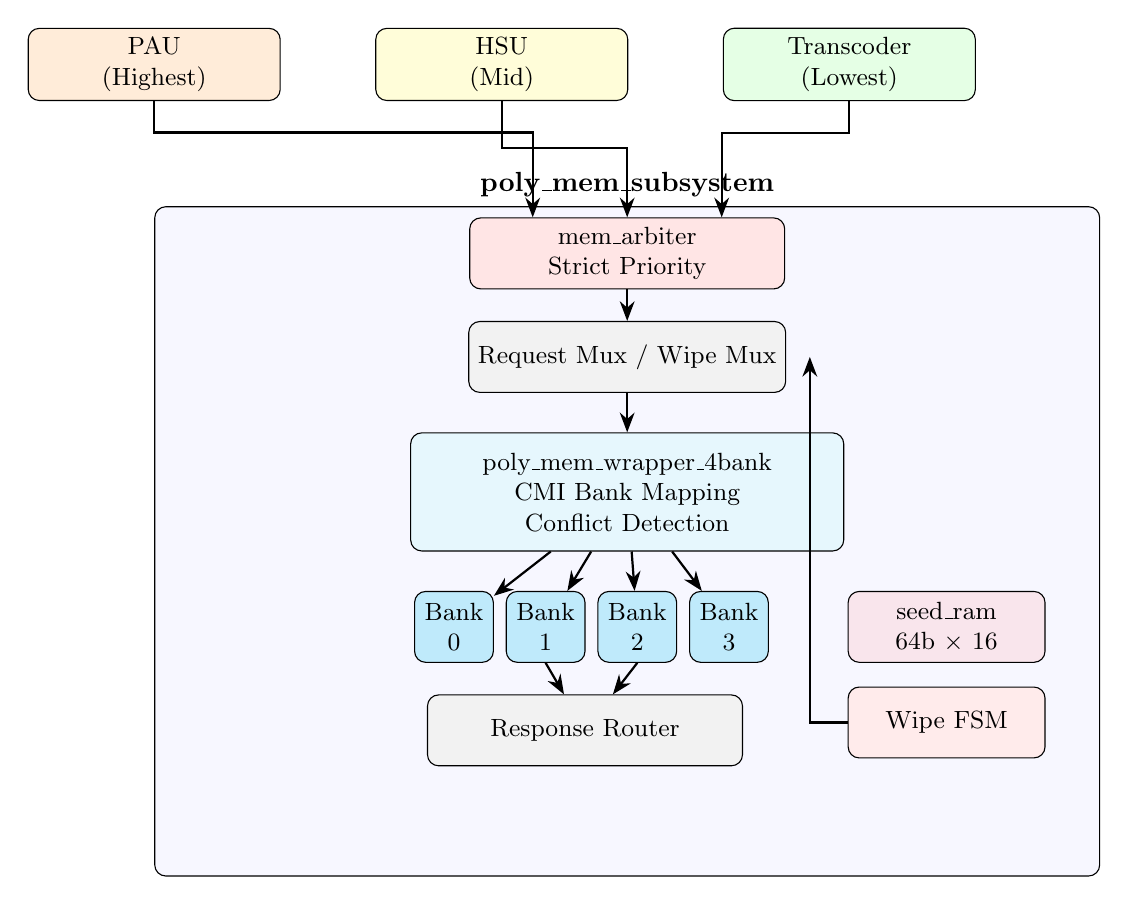
\begin{tikzpicture}[
  block/.style={draw, rounded corners, minimum width=3.2cm,
                minimum height=0.9cm, font=\small, align=center},
  bigblock/.style={draw, rounded corners, minimum width=12cm,
                   minimum height=8.5cm, fill=blue!3},
  arr/.style={-{Stealth[length=2.5mm]}, thick},
  node distance=0.6cm
]

% Outer box
\node[bigblock, label={[font=\bfseries]above:poly\_mem\_subsystem}] (outer) {};

% Clients
\node[block, fill=orange!15] (pau) at ([yshift=1.8cm]outer.north west)
  {PAU\\(Highest)};
\node[block, fill=yellow!15, right=1.2cm of pau] (hsu)
  {HSU\\(Mid)};
\node[block, fill=green!10, right=1.2cm of hsu] (tr)
  {Transcoder\\(Lowest)};

% Arbiter
\node[block, fill=red!10, minimum width=4cm]
  (arb) at ([yshift=-0.6cm]outer.north) {mem\_arbiter\\Strict Priority};

% Request mux
\node[block, fill=gray!10, minimum width=4cm, below=0.4cm of arb]
  (mux) {Request Mux / Wipe Mux};

% Poly wrapper
\node[block, fill=cyan!10, minimum width=5.5cm, minimum height=1.5cm,
      below=0.5cm of mux]
  (wrap) {poly\_mem\_wrapper\_4bank\\CMI Bank Mapping\\Conflict Detection};

% Banks
\node[block, fill=cyan!25, minimum width=1cm, below=0.5cm of wrap,
      xshift=-2.2cm] (b0) {Bank\\0};
\node[block, fill=cyan!25, minimum width=1cm, right=0.15cm of b0] (b1) {Bank\\1};
\node[block, fill=cyan!25, minimum width=1cm, right=0.15cm of b1] (b2) {Bank\\2};
\node[block, fill=cyan!25, minimum width=1cm, right=0.15cm of b2] (b3) {Bank\\3};

% Seed RAM
\node[block, fill=purple!10, minimum width=2.5cm, right=1cm of b3]
  (seed) {seed\_ram\\64b $\times$ 16};

% Wipe FSM
\node[block, fill=red!8, minimum width=2.5cm, below=0.3cm of seed]
  (wipe) {Wipe FSM};

% Response router
\node[block, fill=gray!10, minimum width=4cm,
      below=0.4cm of b1, xshift=0.5cm]
  (rsp) {Response Router};

% Arrows
\draw[arr] (pau.south) -- ++(0,-0.4) -| ([xshift=-1.2cm]arb.north);
\draw[arr] (hsu.south) -- ++(0,-0.6) -| (arb.north);
\draw[arr] (tr.south) -- ++(0,-0.4) -| ([xshift=1.2cm]arb.north);
\draw[arr] (arb) -- (mux);
\draw[arr] (mux) -- (wrap);
\draw[arr] (wrap) -- (b0);
\draw[arr] (wrap) -- (b1);
\draw[arr] (wrap) -- (b2);
\draw[arr] (wrap) -- (b3);
\draw[arr] (b1.south) -- (rsp);
\draw[arr] (b2.south) -- (rsp);
\draw[arr] (wipe.west) -| ([xshift=0.3cm]mux.east);

\end{tikzpicture}
\caption{Top-level architecture of \texttt{poly\_mem\_subsystem}.}
\label{fig:arch}
\end{figure}

% ════════════════════════════════════════════════════════════════
\section{Conflict-Free Memory Interface (CMI) Bank Mapping}
\label{sec:cmi}

\subsection{Motivation}

The NTT butterfly operation reads two coefficients whose indices differ by
a power-of-two stride. Under a simple modulo-4 bank mapping
($\text{bank} = \text{idx} \bmod 4$), many butterfly pairs map to the
same bank. For example, indices 0 and 4 both land in bank~0, forcing the
memory to serialize the access.

\subsection{Bit-Pair-Sum Scheme}

The CMI scheme partitions the 8-bit coefficient index into four 2-bit
fields and sums them modulo~4:

\begin{equation}
  \text{bank} = \bigl(\text{idx}[1{:}0] + \text{idx}[3{:}2]
                     + \text{idx}[5{:}4] + \text{idx}[7{:}6]\bigr) \bmod 4
  \label{eq:cmi}
\end{equation}

This mapping guarantees that every NTT butterfly pair at every stage
(stride 1 through 128) maps to \textbf{distinct banks}, enabling
conflict-free parallel reads.

The row within a bank is simply:
\begin{equation}
  \text{row} = \lfloor \text{idx} / 4 \rfloor
\end{equation}

And the final bank address is:
\begin{equation}
  \text{bank\_addr} = \text{poly\_id} \times \frac{N}{4} + \text{row}
\end{equation}

\subsection{Verification}

The CMI mapping is implemented as a combinational function
\texttt{cmi\_bank\_idx()} inside \texttt{poly\_mem\_wrapper\_4bank.sv}:

\begin{lstlisting}[style=sv, caption={CMI bank mapping function.}]
function automatic [1:0] cmi_bank_idx(
  input logic [$clog2(N)-1:0] order
);
  logic [3:0] sum;
  begin
    sum = order[1:0] + order[3:2]
        + order[5:4] + order[7:6];
    cmi_bank_idx = sum[1:0];
  end
endfunction
\end{lstlisting}

Table~\ref{tab:cmi_example} shows the mapping for the first 12
coefficients, demonstrating that every consecutive group of~4 indices
lands in distinct banks.

\begin{table}[H]
\centering
\caption{CMI bank mapping for indices 0--11.}
\label{tab:cmi_example}
\begin{tabular}{@{}cccccc@{}}
\toprule
\textbf{idx} & \textbf{idx[1:0]} & \textbf{idx[3:2]} &
\textbf{idx[5:4]} & \textbf{idx[7:6]} & \textbf{bank} \\
\midrule
0  & 0 & 0 & 0 & 0 & 0 \\
1  & 1 & 0 & 0 & 0 & 1 \\
2  & 2 & 0 & 0 & 0 & 2 \\
3  & 3 & 0 & 0 & 0 & 3 \\
4  & 0 & 1 & 0 & 0 & 1 \\
5  & 1 & 1 & 0 & 0 & 2 \\
6  & 2 & 1 & 0 & 0 & 3 \\
7  & 3 & 1 & 0 & 0 & 0 \\
8  & 0 & 2 & 0 & 0 & 2 \\
9  & 1 & 2 & 0 & 0 & 3 \\
10 & 2 & 2 & 0 & 0 & 0 \\
11 & 3 & 2 & 0 & 0 & 1 \\
\bottomrule
\end{tabular}
\end{table}

% ════════════════════════════════════════════════════════════════
\section{Polynomial Memory Organization}
\label{sec:poly_org}

\subsection{Per-Polynomial Layout}

Each polynomial contains $N = 256$ coefficients, each $W = 16$ bits wide.
The 256 coefficients are distributed across 4~banks with 64~rows per bank
per polynomial.

\subsection{Multi-Polynomial Storage}

The default configuration provides 32~polynomial slots. The slot
allocation is defined in \texttt{qrem\_mem\_map\_pkg.sv}:

\begin{table}[H]
\centering
\caption{Polynomial slot allocation.}
\label{tab:poly_map}
\begin{tabular}{@{}llcl@{}}
\toprule
\textbf{Region} & \textbf{poly\_id} & \textbf{Count} & \textbf{Purpose} \\
\midrule
A matrix     & 0--15  & 16 & Public matrix (ML-KEM-1024 worst case $4 \times 4$) \\
Secret $s$   & 16--19 & 4  & Secret vector \\
Error $e$    & 20--23 & 4  & Error vector \\
Output $t$   & 24--27 & 4  & Public key / ciphertext result \\
Temp/scratch & 28--31 & 4  & Intermediate storage \\
\bottomrule
\end{tabular}
\end{table}

Each bank therefore has a total depth of:
\begin{equation}
  \text{BANK\_DEPTH} = \text{NUM\_POLYS} \times \frac{N}{4}
                     = 32 \times 64 = 2048 \text{ entries}
\end{equation}

% ════════════════════════════════════════════════════════════════
\section{RTL Module Descriptions}
\label{sec:modules}

\subsection{\texttt{poly\_mem\_subsystem} --- Top-Level Module}

This is the single top-level module that integrates all sub-components.
Its responsibilities are:

\begin{enumerate}
  \item \textbf{Arbitration:} Instantiates \texttt{mem\_arbiter} to
    resolve contention among PAU, HSU, and Transcoder.
  \item \textbf{Request multiplexing:} Routes the winning client's
    4-lane vector request to \texttt{poly\_mem\_wrapper\_4bank}.
  \item \textbf{Wipe multiplexing:} During a security wipe, overrides
    client requests with wipe-generated zero-write commands.
  \item \textbf{Response routing:} Tags each accepted read with an
    \emph{owner ID} and, one cycle later, delivers the response
    exclusively to the originating client.
  \item \textbf{Seed port:} Provides an independent read/write path
    to \texttt{seed\_ram}, unaffected by polynomial arbitration.
  \item \textbf{Security wipe FSM:} Sequences through WIPE\_POLY
    (zeroes all 32 polynomials $\times$ 64 rows), WIPE\_SEED (zeroes
    all 16 seed locations), and WIPE\_DONE.
\end{enumerate}

\subsubsection{Per-Client Interface}

Every client port presents an identical set of signals (Table~\ref{tab:client_if}).

\begin{table}[H]
\centering
\caption{Per-client interface signals (PAU/HSU/Transcoder).}
\label{tab:client_if}
\begin{tabular}{@{}llcl@{}}
\toprule
\textbf{Signal} & \textbf{Dir} & \textbf{Width} & \textbf{Description} \\
\midrule
\texttt{*\_req}            & in  & 1        & Request valid \\
\texttt{*\_poly\_id}       & in  & 5        & Polynomial slot selector \\
\texttt{*\_rd\_en}         & in  & 1        & Read enable \\
\texttt{*\_rd\_idx}        & in  & $4\times8$ & Read coefficient indices \\
\texttt{*\_rd\_lane\_valid} & in & 4        & Per-lane read valid \\
\texttt{*\_wr\_en}         & in  & 4        & Per-lane write enable \\
\texttt{*\_wr\_idx}        & in  & $4\times8$ & Write coefficient indices \\
\texttt{*\_wr\_data}       & in  & $4\times16$ & Write data \\
\texttt{*\_rd\_valid}      & out & 1        & Read response valid (1 cycle later) \\
\texttt{*\_rd\_data}       & out & $4\times16$ & Read data \\
\texttt{*\_stall}          & out & 1        & Client must hold its request \\
\bottomrule
\end{tabular}
\end{table}

\subsubsection{Security Wipe FSM}

\begin{table}[H]
\centering
\caption{Wipe FSM states.}
\label{tab:wipe}
\begin{tabular}{@{}ll@{}}
\toprule
\textbf{State} & \textbf{Action} \\
\midrule
\texttt{WIPE\_IDLE} & Normal operation; transitions on \texttt{wipe\_i} pulse \\
\texttt{WIPE\_POLY} & Writes zero to all $32 \times 64 = 2048$ rows
                       (4 coefficients per cycle, conflict-free) \\
\texttt{WIPE\_SEED} & Writes zero to all 16 seed entries \\
\texttt{WIPE\_DONE} & Asserts \texttt{wipe\_done\_o}; returns to IDLE \\
\bottomrule
\end{tabular}
\end{table}

Total wipe latency:
\begin{equation}
  T_{\text{wipe}} = 32 \times 64 + 16 + 1 = 2065 \text{ cycles}
\end{equation}

During wipe, all client requests are gated and stalled. The wipe writes
consecutive groups of~4 indices per cycle, which always map to distinct
banks under the CMI scheme, so no write conflicts can occur.

% ────────────────────────────────────────────────────────────
\subsection{\texttt{mem\_arbiter} --- Priority Arbitrator}

A purely combinational module implementing strict fixed-priority
arbitration:

\begin{enumerate}
  \item If \texttt{pau\_req\_i} $\rightarrow$ grant PAU; stall HSU and
    Transcoder.
  \item Else if \texttt{hsu\_req\_i} $\rightarrow$ grant HSU; stall
    Transcoder.
  \item Else if \texttt{tr\_req\_i} $\rightarrow$ grant Transcoder.
\end{enumerate}

The winning client sees downstream stall if the memory wrapper reports
\texttt{ready\_o}~$=$~0 (bank conflict). Losing clients always have
\texttt{stall}~$=$~1.

\textbf{Why strict priority?} The PAU sits on the critical path of NTT
and CWM operations, which dominate ML-KEM's cycle count. Guaranteeing
zero additional latency for the PAU maximizes overall throughput. The HSU
and Transcoder operate in phases where the PAU is typically idle, so
starvation is not a practical concern.

% ────────────────────────────────────────────────────────────
\subsection{\texttt{poly\_mem\_wrapper\_4bank} --- 4-Bank Polynomial
Memory}

Implements Poly Port~A (read path) and Poly Port~B (write path) to the
four banked \texttt{poly\_ram\_bank} instances.

\begin{itemize}
  \item \textbf{Bank mapping:} Uses \texttt{cmi\_bank\_idx()} to compute
    the target bank and \texttt{cmi\_bank\_addr()} for the local address.
  \item \textbf{Conflict detection:} Performs 6~pairwise comparisons
    among active read lanes and 6~among active write lanes. If any
    same-bank collision is found, \texttt{ready\_o}~$=$~0 and the
    request is rejected. Read-vs-write same-bank is \emph{not} a
    conflict because they use different RAM ports.
  \item \textbf{Request routing:} Reads are routed to Port~A of the
    target bank; writes to Port~B.
  \item \textbf{Response pipeline:} A single stage of registers captures
    the accepted read's metadata (polynomial~ID, lane indices, bank
    tags). On the next cycle, the response combinator reorders bank
    outputs into lane order using the saved bank tags.
\end{itemize}

% ────────────────────────────────────────────────────────────
\subsection{\texttt{poly\_ram\_bank} --- Dual-Port RAM Primitive}

A single dual-port synchronous RAM. Each instance stores
$\text{BANK\_DEPTH} = 2048$ entries of $W = 16$~bits (default
configuration).

\begin{itemize}
  \item \textbf{Port~A:} Used for reads. Address applied on cycle~$n$;
    data available on cycle~$n{+}1$.
  \item \textbf{Port~B:} Used for writes. Write-enable, address, and data
    applied on the rising clock edge.
  \item Both ports operate independently---simultaneous read on A and
    write on B (even to the same address) is supported.
\end{itemize}

% ────────────────────────────────────────────────────────────
\subsection{\texttt{seed\_ram} --- Seed and Protocol Store}

A simple synchronous RAM for storing cryptographic seeds, hash state,
and protocol metadata.

\begin{itemize}
  \item Default: 16~entries $\times$ 64~bits.
  \item 1-cycle read latency (synchronous read).
  \item Independent request port on \texttt{poly\_mem\_subsystem}; not
    subject to PAU/HSU/Transcoder arbitration.
  \item Zeroed by the wipe FSM during the \texttt{WIPE\_SEED} phase.
\end{itemize}

% ────────────────────────────────────────────────────────────
\subsection{\texttt{delay\_n} --- Generic Delay Line}

A parameterized shift register used inside the CMI module
(\texttt{cmi.sv}) to align writeback indices with Arithmetic Unit result
data. Instantiated at depths 2, 4, 5, and 9~cycles corresponding to the
latencies of different PAU operations (NTT butterfly, CWM, ADD drain).

% ────────────────────────────────────────────────────────────
\subsection{\texttt{cmi.sv} --- Conflict-Free Memory Interface (PAU
Component)}

\textbf{Note:} This module belongs to the PAU, not the Memory Subsystem.
It is included in the repository to define the interface contract between
the PAU and \texttt{poly\_mem\_wrapper\_4bank}.

\begin{itemize}
  \item Forwards 4-lane read requests (coefficient indices $+$ valid
    flags) to the memory wrapper.
  \item Consumes the wrapper's 1-cycle read response and presents aligned
    coefficient data to the Arithmetic Unit.
  \item Aligns writeback addresses via configurable \texttt{delay\_n}
    pipelines so write indices arrive at the wrapper simultaneously with
    AU result data.
  \item Supports write-only cycles (no concurrent read) for drain/final
    writeback phases.
\end{itemize}

% ────────────────────────────────────────────────────────────
\subsection{\texttt{qrem\_mem\_map\_pkg} --- Polynomial Slot Map}

A SystemVerilog package defining \texttt{localparam} constants for the
32-polynomial address map (Table~\ref{tab:poly_map}). The system
controller uses these constants to address specific polynomial slots
during NTT, sampling, encoding, and key generation.

% ════════════════════════════════════════════════════════════════
\section{Read/Write Timing}
\label{sec:timing}

\begin{table}[H]
\centering
\caption{Read and write timing diagram.}
\label{tab:timing}
\begin{tabular}{@{}cll@{}}
\toprule
\textbf{Cycle} & \textbf{Read Path} & \textbf{Write Path} \\
\midrule
0 & Client asserts \texttt{req}, \texttt{rd\_en}, \texttt{rd\_idx}
  & Client asserts \texttt{wr\_en}, \texttt{wr\_idx}, \texttt{wr\_data} \\
  & Arbiter grants; wrapper accepts (\texttt{ready\_o}=1)
  & Write applied to Port~B on clock edge \\
  & Port~A address applied to bank RAM
  & \\
\midrule
1 & Bank RAM outputs data on \texttt{a\_rdata}
  & Write data visible to subsequent reads \\
  & Wrapper presents \texttt{rd\_valid\_o}=1
  & \\
  & \texttt{poly\_mem\_subsystem} routes to originating client
  & \\
\bottomrule
\end{tabular}
\end{table}

% ════════════════════════════════════════════════════════════════
\section{Conflict Detection}
\label{sec:conflict}

Bank conflicts occur when two active read lanes (or two active write
lanes) target the same bank in the same cycle. The wrapper performs
$\binom{4}{2} = 6$ pairwise comparisons for reads and 6 for writes:

\begin{lstlisting}[style=sv, caption={Conflict detection excerpt.}]
if (rd_lane_valid_i[0] && rd_lane_valid_i[1]
    && (rd_bank[0] == rd_bank[1]))
  rd_conflict = 1'b1;
// ... 5 more pairs ...
\end{lstlisting}

When a conflict is detected:
\begin{itemize}
  \item \texttt{ready\_o} is deasserted.
  \item The request is \emph{not} accepted (no RAM access occurs).
  \item The arbiter propagates the stall to the requesting client.
  \item The client must hold its request until \texttt{stall} is released.
\end{itemize}

Read-vs-write to the same bank is \textbf{not} a conflict because reads
use Port~A and writes use Port~B of the dual-port RAM.

% ════════════════════════════════════════════════════════════════
\section{Security Wipe}
\label{sec:wipe}

FIPS~203 requires that implementations securely erase intermediate
key material after use. The wipe FSM provides a hardware-level guarantee:

\begin{enumerate}
  \item A single-cycle pulse on \texttt{wipe\_i} initiates the wipe.
  \item \textbf{WIPE\_POLY:} The FSM iterates over all 32~polynomials
    $\times$ 64 rows, writing 4~zero coefficients per cycle. Under the
    CMI mapping, consecutive groups of~4 indices always land in distinct
    banks, so no write conflict occurs and \texttt{ready\_o} remains
    high throughout.
  \item \textbf{WIPE\_SEED:} The FSM zeroes all 16 seed RAM locations.
  \item \textbf{WIPE\_DONE:} Asserts \texttt{wipe\_done\_o} for one cycle
    and returns to idle.
  \item All client requests are gated (forced stall) for the entire
    duration of the wipe.
\end{enumerate}

% ════════════════════════════════════════════════════════════════
\section{Simulation and Verification}
\label{sec:sim}

The project includes a shared Makefile supporting both ModelSim/Questa
and Verilator:

\begin{lstlisting}[language=bash, style=sv, caption={Running testbenches.}]
# Run all testbenches with Verilator
make run_all SIM=verilator

# Run a single testbench
make run_poly_mem_tb SIM=verilator
make run_mem_frontend_top_tb SIM=verilator
\end{lstlisting}

\begin{table}[H]
\centering
\caption{Testbench coverage summary.}
\label{tab:tb}
\begin{tabular}{@{}ll@{}}
\toprule
\textbf{Testbench} & \textbf{Verified Functionality} \\
\midrule
\texttt{poly\_mem\_tb}
  & PAU smoke test: write/read, seed store, wipe \\
\texttt{mem\_frontend\_top\_tb}
  & Full integration: all 3 clients, arbitration, isolation, wipe \\
\texttt{poly\_mem\_wrapper\_4bank\_tb}
  & CMI mapping, conflict detection, read reorder \\
\texttt{cmi\_tb}
  & Read forwarding, writeback delay alignment \\
\texttt{mem\_arbiter\_tb}
  & Priority ordering, stall propagation \\
\texttt{seed\_ram\_tb}
  & Write/read, address sweep \\
\bottomrule
\end{tabular}
\end{table}

All testbenches output \texttt{TB PASS} upon successful completion.

% ════════════════════════════════════════════════════════════════
\section{Directory Structure}
\label{sec:dir}

\begin{lstlisting}[basicstyle=\ttfamily\small, frame=none, numbers=none]
poly-mem-subsystem/
  rtl/
    qrem_mem_map_pkg.sv
    delay_n.sv
    cmi.sv
    mem_arbiter.sv
    poly_ram_bank.sv
    seed_ram.sv
    poly_mem_wrapper_4bank.sv
    poly_mem_subsystem.sv        (top-level)
  tb/
    poly_mem_tb.sv
    mem_frontend_top_tb.sv
    poly_mem_wrapper_4bank_tb.sv
    cmi_tb.sv
    mem_arbiter_tb.sv
    seed_ram_tb.sv
  doc/
    docs.md
    memory_subsystem.tex         (this document)
  build-tools/
  rtl.f
  Makefile
  README.md
\end{lstlisting}

% ════════════════════════════════════════════════════════════════
\section{Summary}
\label{sec:summary}

The QREM polynomial memory subsystem provides:

\begin{itemize}
  \item A \textbf{four-bank dual-port polynomial memory} with CMI
    conflict-free bank mapping ensuring zero-conflict NTT butterfly
    access.
  \item A \textbf{strict-priority arbiter} (PAU~$>$~HSU~$>$~Transcoder)
    granting exactly one client per cycle with stall-based flow control.
  \item \textbf{Deterministic 1-cycle read latency} with tagged response
    routing that guarantees each client only receives its own read data.
  \item A \textbf{dedicated seed/protocol store} on an independent port.
  \item A \textbf{hardware security-wipe FSM} clearing all 32~polynomials
    and 16~seed locations in approximately 2065~cycles.
  \item \textbf{32-polynomial capacity} organized via a configurable
    address map supporting ML-KEM-512/768/1024 parameter sets.
\end{itemize}

The architecture follows the Memory Subsystem design described in
\emph{``Highly-Efficient Hardware Architecture for ML-KEM PQC Standard''}
(IEEE OJCAS, 2025) and is fully verified by six independent testbenches
at the unit, integration, and system levels.

\end{document}
